\section{Results}

\begin{figure*}[!t]
  \resizebox{\textwidth}{!}{
    \subfloat{
      \myboxplot{
% L: 0
\addplot[mark=*,boxplot, boxplot/draw position=0]
table[row sep=\\, y index=0] {
data
0.52 \\
0.52 \\
0.48 \\
0.52 \\
0.52 \\
0.48 \\
0.52 \\
0.52 \\
0.52 \\
0.52 \\
0.47 \\
0.52 \\
0.56 \\
0.52 \\
0.47 \\
0.52 \\
0.52 \\
0.52 \\
0.52 \\
0.52 \\
0.47 \\
0.52 \\
0.48 \\
0.47 \\
0.52 \\
0.43 \\
0.52 \\
0.52 \\
0.47 \\
0.52 \\
};
% L: 1
\addplot[mark=*,boxplot, boxplot/draw position=1]
table[row sep=\\, y index=0] {
data
0.55 \\
0.465 \\
0.47 \\
0.36 \\
0.48 \\
0.465 \\
0.47 \\
0.425 \\
0.47 \\
0.455 \\
0.485 \\
0.475 \\
0.48 \\
0.44 \\
0.465 \\
0.645 \\
0.47 \\
0.48 \\
0.36 \\
0.48 \\
0.36 \\
0.48 \\
0.48 \\
0.465 \\
0.52 \\
0.48 \\
0.495 \\
0.48 \\
0.36 \\
0.475 \\
};
% L: 2
\addplot[mark=*,boxplot, boxplot/draw position=2]
table[row sep=\\, y index=0] {
data
0.465 \\
0.465 \\
0.47 \\
0.36 \\
0.36 \\
0.475 \\
0.48 \\
0.49 \\
0.51 \\
0.48 \\
0.475 \\
0.465 \\
0.465 \\
0.47 \\
0.475 \\
0.465 \\
0.475 \\
0.515 \\
0.48 \\
0.475 \\
0.465 \\
0.465 \\
0.475 \\
0.455 \\
0.455 \\
0.48 \\
0.48 \\
0.475 \\
0.47 \\
0.49 \\
};
% L: 3
\addplot[mark=*,boxplot, boxplot/draw position=3]
table[row sep=\\, y index=0] {
data
0.41 \\
0.47 \\
0.405 \\
0.405 \\
0.54 \\
0.475 \\
0.48 \\
0.5 \\
0.5 \\
0.48 \\
0.4 \\
0.45 \\
0.425 \\
0.485 \\
0.465 \\
0.445 \\
0.355 \\
0.465 \\
0.47 \\
0.475 \\
0.595 \\
0.485 \\
0.525 \\
0.61 \\
0.475 \\
0.645 \\
0.36 \\
0.475 \\
0.49 \\
0.465 \\
};
% L: 4
\addplot[mark=*,boxplot, boxplot/draw position=4]
table[row sep=\\, y index=0] {
data
0.465 \\
0.585 \\
0.645 \\
0.405 \\
0.475 \\
0.465 \\
0.485 \\
0.36 \\
0.465 \\
0.48 \\
0.475 \\
0.545 \\
0.465 \\
0.41 \\
0.485 \\
0.475 \\
0.47 \\
0.465 \\
0.595 \\
0.465 \\
0.41 \\
0.47 \\
0.47 \\
0.495 \\
0.485 \\
0.49 \\
0.465 \\
0.475 \\
0.48 \\
0.48 \\
};
% L: 5
\addplot[mark=*,boxplot, boxplot/draw position=5]
table[row sep=\\, y index=0] {
data
0.465 \\
0.465 \\
0.465 \\
0.57 \\
0.36 \\
0.475 \\
0.465 \\
0.475 \\
0.435 \\
0.475 \\
0.53 \\
0.465 \\
0.48 \\
0.355 \\
0.555 \\
0.47 \\
0.475 \\
0.455 \\
0.465 \\
0.475 \\
0.475 \\
0.475 \\
0.475 \\
0.52 \\
0.425 \\
0.585 \\
0.465 \\
0.465 \\
0.405 \\
0.485 \\
};
% L: 6
\addplot[mark=*,boxplot, boxplot/draw position=6]
table[row sep=\\, y index=0] {
data
0.465 \\
0.54 \\
0.54 \\
0.47 \\
0.475 \\
0.435 \\
0.475 \\
0.405 \\
0.355 \\
0.465 \\
0.465 \\
0.465 \\
0.465 \\
0.47 \\
0.41 \\
0.465 \\
0.465 \\
0.465 \\
0.475 \\
0.475 \\
0.465 \\
0.46 \\
0.645 \\
0.465 \\
0.465 \\
0.475 \\
0.475 \\
0.475 \\
0.465 \\
};
% L: 7
\addplot[mark=*,boxplot, boxplot/draw position=7]
table[row sep=\\, y index=0] {
data
0.465 \\
0.465 \\
0.475 \\
0.645 \\
0.475 \\
0.475 \\
0.465 \\
0.465 \\
0.48 \\
0.465 \\
0.475 \\
0.465 \\
0.395 \\
0.465 \\
0.475 \\
0.465 \\
0.645 \\
0.465 \\
0.475 \\
0.47 \\
0.48 \\
0.475 \\
0.47 \\
0.425 \\
0.475 \\
0.465 \\
0.465 \\
0.475 \\
0.47 \\
0.465 \\
};
% L: 8
\addplot[mark=*,boxplot, boxplot/draw position=8]
table[row sep=\\, y index=0] {
data
0.465 \\
0.465 \\
0.465 \\
0.465 \\
0.465 \\
0.475 \\
0.465 \\
0.465 \\
0.465 \\
0.465 \\
0.475 \\
0.465 \\
0.475 \\
0.465 \\
0.465 \\
0.48 \\
0.465 \\
0.465 \\
0.475 \\
0.465 \\
0.47 \\
0.475 \\
0.465 \\
0.475 \\
0.465 \\
0.465 \\
0.465 \\
0.475 \\
0.465 \\
0.475 \\
};
% L: 9
\addplot[mark=*,boxplot, boxplot/draw position=9]
table[row sep=\\, y index=0] {
data
0.475 \\
0.465 \\
0.475 \\
0.36 \\
0.465 \\
0.535 \\
0.465 \\
0.465 \\
0.535 \\
0.475 \\
0.465 \\
0.595 \\
0.475 \\
0.465 \\
0.475 \\
0.475 \\
0.465 \\
0.475 \\
0.475 \\
0.475 \\
0.465 \\
0.465 \\
0.475 \\
0.475 \\
0.475 \\
0.475 \\
0.465 \\
0.535 \\
0.475 \\
0.535 \\
};
% L: 10
\addplot[mark=*,boxplot, boxplot/draw position=10]
table[row sep=\\, y index=0] {
data
0.535 \\
0.535 \\
0.535 \\
0.535 \\
0.535 \\
0.535 \\
0.535 \\
0.535 \\
0.535 \\
0.535 \\
0.535 \\
0.535 \\
0.535 \\
0.535 \\
0.535 \\
0.535 \\
0.535 \\
0.535 \\
0.535 \\
0.535 \\
0.535 \\
0.535 \\
0.535 \\
0.535 \\
0.535 \\
0.535 \\
0.535 \\
0.535 \\
0.535 \\
0.535 \\
};
}{0.1}

    }
    \subfloat{
      \myboxplot{
% L: 0
\addplot[
boxplot prepared={
    draw position=0,
    median=0.525,
    upper quartile=0.525,
    lower quartile=0.521,
    upper whisker=0.525,
    lower whisker=0.525
},
] coordinates {};
% L: 10
\addplot[
boxplot prepared={
    draw position=1,
    median=0.5175,
    upper quartile=0.575,
    lower quartile=0.48,
    upper whisker=0.775,
    lower whisker=0.455
},
] coordinates {};
% L: 20
\addplot[
boxplot prepared={
    draw position=2,
    median=0.6625,
    upper quartile=0.92375,
    lower quartile=0.51875,
    upper whisker=1.0,
    lower whisker=0.46
},
] coordinates {};
% L: 30
\addplot[
boxplot prepared={
    draw position=3,
    median=0.8975,
    upper quartile=1.0,
    lower quartile=0.5275,
    upper whisker=1.0,
    lower whisker=0.445
},
] coordinates {};
% L: 40
\addplot[
boxplot prepared={
    draw position=4,
    median=1.0,
    upper quartile=1.0,
    lower quartile=0.84875,
    upper whisker=1.0,
    lower whisker=0.435
},
] coordinates {};
% L: 50
\addplot[
boxplot prepared={
    draw position=5,
    median=1.0,
    upper quartile=1.0,
    lower quartile=0.996,
    upper whisker=1.0,
    lower whisker=0.615
},
] coordinates {};
% L: 60
\addplot[
boxplot prepared={
    draw position=6,
    median=1.0,
    upper quartile=1.0,
    lower quartile=0.996,
    upper whisker=1.0,
    lower whisker=0.33
},
] coordinates {};
% L: 70
\addplot[
boxplot prepared={
    draw position=7,
    median=0.875,
    upper quartile=1.0,
    lower quartile=0.54125,
    upper whisker=1.0,
    lower whisker=0.31
},
] coordinates {};
% L: 80
\addplot[
boxplot prepared={
    draw position=8,
    median=0.7625,
    upper quartile=0.92375,
    lower quartile=0.51125,
    upper whisker=1.0,
    lower whisker=0.355
},
] coordinates {};
% L: 90
\addplot[
boxplot prepared={
    draw position=9,
    median=0.51,
    upper quartile=0.74,
    lower quartile=0.51,
    upper whisker=1.0,
    lower whisker=0.505
},
] coordinates {};
% L: 100
\addplot[
boxplot prepared={
    draw position=10,
    median=0.51,
    upper quartile=0.51,
    lower quartile=0.506,
    upper whisker=0.51,
    lower whisker=0.51
},
] coordinates {};
}{0.1}

    }
    \subfloat{
      \myboxplot{
% L: 0
\addplot[mark=*, boxplot]
table[row sep=\\, y index=0] {
data
0.525 \\
0.455 \\
0.515 \\
0.535 \\
0.525 \\
0.51 \\
0.58 \\
0.525 \\
0.495 \\
0.505 \\
0.51 \\
0.575 \\
0.49 \\
0.425 \\
0.545 \\
0.5 \\
0.52 \\
0.48 \\
0.495 \\
0.455 \\
0.54 \\
0.53 \\
0.49 \\
0.44 \\
0.52 \\
0.485 \\
0.455 \\
0.535 \\
0.51 \\
0.54 \\
};
% L: 1
\addplot[mark=*, boxplot]
table[row sep=\\, y index=0] {
data
0.72 \\
0.71 \\
0.68 \\
0.45 \\
0.575 \\
0.545 \\
0.535 \\
0.54 \\
0.645 \\
0.58 \\
0.695 \\
0.57 \\
0.75 \\
0.48 \\
0.67 \\
0.48 \\
0.505 \\
0.57 \\
0.56 \\
0.64 \\
0.6 \\
0.61 \\
0.515 \\
0.585 \\
0.515 \\
0.49 \\
0.51 \\
0.615 \\
0.74 \\
0.6 \\
};
% L: 2
\addplot[mark=*, boxplot]
table[row sep=\\, y index=0] {
data
0.9 \\
0.725 \\
0.565 \\
0.73 \\
0.665 \\
0.805 \\
0.9 \\
0.785 \\
0.77 \\
0.81 \\
0.95 \\
0.675 \\
0.71 \\
0.835 \\
0.6 \\
0.71 \\
0.725 \\
0.64 \\
0.74 \\
0.755 \\
0.75 \\
0.875 \\
0.7 \\
0.77 \\
0.72 \\
0.805 \\
0.57 \\
0.76 \\
0.77 \\
0.63 \\
};
% L: 3
\addplot[mark=*, boxplot]
table[row sep=\\, y index=0] {
data
0.81 \\
0.99 \\
0.945 \\
0.905 \\
0.935 \\
0.965 \\
0.905 \\
0.905 \\
0.98 \\
0.99 \\
0.955 \\
0.99 \\
0.99 \\
0.94 \\
0.77 \\
0.99 \\
0.755 \\
0.98 \\
0.705 \\
0.88 \\
0.755 \\
0.965 \\
0.975 \\
0.735 \\
0.92 \\
0.93 \\
};
% L: 4
\addplot[mark=*, boxplot]
table[row sep=\\, y index=0] {
data
0.99 \\
0.99 \\
0.985 \\
0.97 \\
0.985 \\
0.91 \\
0.975 \\
0.99 \\
0.99 \\
0.98 \\
0.99 \\
0.99 \\
0.965 \\
0.99 \\
0.99 \\
0.99 \\
0.99 \\
0.985 \\
0.985 \\
0.905 \\
0.905 \\
0.985 \\
0.98 \\
0.99 \\
0.97 \\
0.96 \\
0.945 \\
0.99 \\
0.95 \\
0.91 \\
};
% L: 5
\addplot[mark=*, boxplot]
table[row sep=\\, y index=0] {
data
0.99 \\
0.99 \\
0.99 \\
0.99 \\
0.99 \\
0.99 \\
0.985 \\
0.99 \\
0.99 \\
0.99 \\
0.99 \\
0.99 \\
0.965 \\
0.955 \\
0.99 \\
0.99 \\
0.99 \\
0.99 \\
0.99 \\
0.985 \\
0.975 \\
0.99 \\
0.99 \\
0.98 \\
0.915 \\
0.99 \\
0.99 \\
0.98 \\
};
% L: 6
\addplot[mark=*, boxplot]
table[row sep=\\, y index=0] {
data
0.99 \\
0.99 \\
0.99 \\
0.99 \\
0.99 \\
0.99 \\
0.49 \\
0.99 \\
0.99 \\
0.99 \\
0.99 \\
0.99 \\
0.99 \\
0.99 \\
0.99 \\
0.99 \\
0.99 \\
0.99 \\
0.97 \\
0.99 \\
0.99 \\
0.99 \\
0.99 \\
0.99 \\
0.99 \\
0.99 \\
0.95 \\
0.99 \\
};
% L: 7
\addplot[mark=*, boxplot]
table[row sep=\\, y index=0] {
data
0.99 \\
0.915 \\
0.99 \\
0.99 \\
0.99 \\
0.99 \\
0.99 \\
0.645 \\
0.99 \\
0.99 \\
0.78 \\
0.95 \\
0.965 \\
0.99 \\
0.99 \\
0.99 \\
0.99 \\
0.99 \\
0.99 \\
0.95 \\
0.99 \\
0.99 \\
0.99 \\
0.99 \\
0.94 \\
0.99 \\
0.99 \\
0.99 \\
0.99 \\
};
% L: 8
\addplot[mark=*, boxplot]
table[row sep=\\, y index=0] {
data
0.99 \\
0.99 \\
0.99 \\
0.99 \\
0.555 \\
0.99 \\
0.99 \\
0.98 \\
0.99 \\
0.835 \\
0.99 \\
0.99 \\
0.99 \\
0.69 \\
0.615 \\
0.645 \\
0.93 \\
0.93 \\
0.99 \\
0.865 \\
0.93 \\
0.865 \\
0.455 \\
0.69 \\
0.99 \\
0.97 \\
0.99 \\
0.99 \\
0.345 \\
};
% L: 9
\addplot[mark=*, boxplot]
table[row sep=\\, y index=0] {
data
0.53 \\
0.69 \\
0.72 \\
0.705 \\
0.42 \\
0.53 \\
0.63 \\
0.69 \\
0.42 \\
0.42 \\
0.99 \\
0.99 \\
0.42 \\
0.305 \\
0.655 \\
0.42 \\
0.62 \\
0.835 \\
0.42 \\
0.42 \\
0.655 \\
0.705 \\
0.49 \\
0.69 \\
0.42 \\
0.42 \\
0.72 \\
};
% L: 10
\addplot[mark=*, boxplot]
table[row sep=\\, y index=0] {
data
0.46 \\
0.46 \\
0.46 \\
0.46 \\
0.46 \\
0.46 \\
0.46 \\
0.46 \\
0.46 \\
0.46 \\
0.46 \\
0.46 \\
0.46 \\
0.46 \\
0.46 \\
0.46 \\
0.46 \\
0.46 \\
0.46 \\
0.46 \\
0.46 \\
0.46 \\
0.46 \\
0.46 \\
0.46 \\
0.46 \\
0.46 \\
0.46 \\
0.46 \\
0.46 \\
};
}{0.1}

    }
  }

  \resizebox{\textwidth}{!}{
    \subfloat{
      \myscatterplot{results/computational-power-100-3-1.dat}
    }
    \subfloat{
      \myscatterplot{results/computational-power-100-3.dat}
    }
    \subfloat{
      \myscatterplot{results/computational-power-100-3-3.dat}
    }
  }
  \caption{Figures a-c show the average performance with K=[1,2,3] for temporal 100 3. We see that 1 sucks a bit compared to 2 and 3, although 2 and 3 both work.}
\end{figure*}

\begin{figure*}[!t]
  \resizebox{\textwidth}{!}{
    \subfloat{
      \myboxplot{
% L: 0
\addplot[mark=*, mark=*,boxplot, boxplot/draw position=0]
table[row sep=\\, y index=0] {
data
0.555 \\
0.555 \\
0.555 \\
0.555 \\
0.555 \\
0.565 \\
0.555 \\
0.555 \\
0.555 \\
0.455 \\
0.555 \\
0.555 \\
0.555 \\
0.455 \\
0.555 \\
0.555 \\
0.555 \\
0.555 \\
0.555 \\
0.455 \\
0.555 \\
0.565 \\
0.555 \\
0.555 \\
0.455 \\
0.555 \\
0.555 \\
0.455 \\
0.455 \\
0.555 \\
};
% L: 1
\addplot[mark=*, mark=*,boxplot, boxplot/draw position=1]
table[row sep=\\, y index=0] {
data
0.49 \\
0.5 \\
0.51 \\
0.55 \\
0.5 \\
0.485 \\
0.495 \\
0.505 \\
0.535 \\
0.535 \\
0.455 \\
0.555 \\
0.455 \\
0.49 \\
0.5 \\
0.545 \\
0.485 \\
0.545 \\
0.555 \\
0.455 \\
0.565 \\
0.535 \\
0.505 \\
0.465 \\
0.565 \\
0.535 \\
0.46 \\
0.555 \\
0.505 \\
0.485 \\
};
% L: 2
\addplot[mark=*, mark=*,boxplot, boxplot/draw position=2]
table[row sep=\\, y index=0] {
data
0.485 \\
0.515 \\
0.515 \\
0.475 \\
0.545 \\
0.485 \\
0.555 \\
0.505 \\
0.555 \\
0.485 \\
0.455 \\
0.505 \\
0.515 \\
0.5 \\
0.555 \\
0.555 \\
0.475 \\
0.485 \\
0.5 \\
0.5 \\
0.51 \\
0.505 \\
0.545 \\
0.555 \\
0.535 \\
0.485 \\
0.555 \\
0.485 \\
0.455 \\
0.46 \\
};
% L: 3
\addplot[mark=*, mark=*,boxplot, boxplot/draw position=3]
table[row sep=\\, y index=0] {
data
0.435 \\
0.485 \\
0.485 \\
0.485 \\
0.485 \\
0.505 \\
0.55 \\
0.535 \\
0.525 \\
0.525 \\
0.545 \\
0.485 \\
0.525 \\
0.525 \\
0.555 \\
0.535 \\
0.455 \\
0.555 \\
0.525 \\
0.515 \\
0.485 \\
0.485 \\
0.485 \\
0.485 \\
0.455 \\
0.545 \\
0.535 \\
0.545 \\
0.555 \\
0.555 \\
};
% L: 4
\addplot[mark=*, mark=*,boxplot, boxplot/draw position=4]
table[row sep=\\, y index=0] {
data
0.485 \\
0.485 \\
0.525 \\
0.485 \\
0.535 \\
0.485 \\
0.485 \\
0.545 \\
0.485 \\
0.485 \\
0.525 \\
0.515 \\
0.535 \\
0.485 \\
0.495 \\
0.455 \\
0.525 \\
0.525 \\
0.485 \\
0.485 \\
0.535 \\
0.485 \\
0.455 \\
0.535 \\
0.48 \\
0.545 \\
0.52 \\
0.525 \\
0.51 \\
0.485 \\
};
% L: 5
\addplot[mark=*, mark=*,boxplot, boxplot/draw position=5]
table[row sep=\\, y index=0] {
data
0.545 \\
0.505 \\
0.515 \\
0.535 \\
0.5 \\
0.555 \\
0.485 \\
0.485 \\
0.455 \\
0.555 \\
0.535 \\
0.485 \\
0.485 \\
0.555 \\
0.485 \\
0.485 \\
0.47 \\
0.555 \\
0.505 \\
0.51 \\
0.51 \\
0.545 \\
0.475 \\
0.545 \\
0.555 \\
0.535 \\
0.485 \\
0.505 \\
0.465 \\
0.485 \\
};
% L: 6
\addplot[mark=*, mark=*,boxplot, boxplot/draw position=6]
table[row sep=\\, y index=0] {
data
0.555 \\
0.485 \\
0.495 \\
0.485 \\
0.495 \\
0.46 \\
0.485 \\
0.555 \\
0.535 \\
0.465 \\
0.555 \\
0.455 \\
0.485 \\
0.535 \\
0.555 \\
0.545 \\
0.485 \\
0.535 \\
0.555 \\
0.495 \\
0.555 \\
0.485 \\
0.525 \\
0.455 \\
0.505 \\
0.485 \\
0.455 \\
0.5 \\
0.48 \\
};
% L: 7
\addplot[mark=*, mark=*,boxplot, boxplot/draw position=7]
table[row sep=\\, y index=0] {
data
0.485 \\
0.555 \\
0.555 \\
0.475 \\
0.555 \\
0.555 \\
0.485 \\
0.555 \\
0.46 \\
0.485 \\
0.455 \\
0.485 \\
0.455 \\
0.555 \\
0.555 \\
0.555 \\
0.485 \\
0.555 \\
0.475 \\
0.455 \\
0.525 \\
0.485 \\
0.485 \\
0.555 \\
0.555 \\
0.535 \\
0.555 \\
0.555 \\
0.455 \\
0.525 \\
};
% L: 8
\addplot[mark=*, mark=*,boxplot, boxplot/draw position=8]
table[row sep=\\, y index=0] {
data
0.455 \\
0.555 \\
0.485 \\
0.485 \\
0.555 \\
0.555 \\
0.485 \\
0.555 \\
0.485 \\
0.505 \\
0.555 \\
0.455 \\
0.555 \\
0.555 \\
0.455 \\
0.555 \\
0.555 \\
0.555 \\
0.555 \\
0.555 \\
0.535 \\
0.555 \\
0.555 \\
0.555 \\
0.555 \\
0.525 \\
0.555 \\
0.555 \\
0.555 \\
};
% L: 9
\addplot[mark=*, mark=*,boxplot, boxplot/draw position=9]
table[row sep=\\, y index=0] {
data
0.555 \\
0.555 \\
0.455 \\
0.555 \\
0.555 \\
0.525 \\
0.485 \\
0.555 \\
0.495 \\
0.535 \\
0.555 \\
0.555 \\
0.555 \\
0.505 \\
0.555 \\
0.525 \\
0.505 \\
0.505 \\
0.555 \\
0.555 \\
0.555 \\
0.555 \\
0.555 \\
0.555 \\
0.555 \\
0.555 \\
0.555 \\
};
% L: 10
\addplot[mark=*, mark=*,boxplot, boxplot/draw position=10]
table[row sep=\\, y index=0] {
data
0.555 \\
0.555 \\
0.555 \\
0.555 \\
0.555 \\
0.555 \\
0.555 \\
0.555 \\
0.555 \\
0.555 \\
0.555 \\
0.555 \\
0.555 \\
0.555 \\
0.555 \\
0.555 \\
0.555 \\
0.555 \\
0.555 \\
0.555 \\
0.555 \\
0.555 \\
0.555 \\
0.555 \\
0.555 \\
0.555 \\
0.555 \\
0.555 \\
0.555 \\
0.555 \\
};
}{0.1}

    }
    \subfloat{
      \myboxplot{
% L: 0
\addplot[
boxplot prepared={
    draw position=0,
    median=0.565,
    upper quartile=0.565,
    lower quartile=0.561,
    upper whisker=0.565,
    lower whisker=0.565
},
] coordinates {};
% L: 10
\addplot[
boxplot prepared={
    draw position=1,
    median=0.55,
    upper quartile=0.56875,
    lower quartile=0.52625,
    upper whisker=0.595,
    lower whisker=0.5
},
] coordinates {};
% L: 20
\addplot[
boxplot prepared={
    draw position=2,
    median=0.535,
    upper quartile=0.57375,
    lower quartile=0.52625,
    upper whisker=0.67,
    lower whisker=0.51
},
] coordinates {};
% L: 30
\addplot[
boxplot prepared={
    draw position=3,
    median=0.5525,
    upper quartile=0.565,
    lower quartile=0.5325,
    upper whisker=0.775,
    lower whisker=0.505
},
] coordinates {};
% L: 40
\addplot[
boxplot prepared={
    draw position=4,
    median=0.5575,
    upper quartile=0.58125,
    lower quartile=0.54125,
    upper whisker=0.985,
    lower whisker=0.51
},
] coordinates {};
% L: 50
\addplot[
boxplot prepared={
    draw position=5,
    median=0.56,
    upper quartile=0.585,
    lower quartile=0.555,
    upper whisker=0.845,
    lower whisker=0.515
},
] coordinates {};
% L: 60
\addplot[
boxplot prepared={
    draw position=6,
    median=0.555,
    upper quartile=0.57375,
    lower quartile=0.555,
    upper whisker=0.75,
    lower whisker=0.52
},
] coordinates {};
% L: 70
\addplot[
boxplot prepared={
    draw position=7,
    median=0.5625,
    upper quartile=0.565,
    lower quartile=0.555,
    upper whisker=0.61,
    lower whisker=0.52
},
] coordinates {};
% L: 80
\addplot[
boxplot prepared={
    draw position=8,
    median=0.565,
    upper quartile=0.565,
    lower quartile=0.555,
    upper whisker=0.605,
    lower whisker=0.545
},
] coordinates {};
% L: 90
\addplot[
boxplot prepared={
    draw position=9,
    median=0.49,
    upper quartile=0.51,
    lower quartile=0.49,
    upper whisker=0.525,
    lower whisker=0.46
},
] coordinates {};
% L: 100
\addplot[
boxplot prepared={
    draw position=10,
    median=0.53,
    upper quartile=0.53,
    lower quartile=0.526,
    upper whisker=0.53,
    lower whisker=0.53
},
] coordinates {};
}{0.1}

    }
    \subfloat{
      \myboxplot{
% L: 0
\addplot[
boxplot prepared={
    draw position=0,
    median=0.465,
    upper quartile=0.465,
    lower quartile=0.461,
    upper whisker=0.465,
    lower whisker=0.465
},
] coordinates {};
% L: 10
\addplot[
boxplot prepared={
    draw position=1,
    median=0.4975,
    upper quartile=0.515,
    lower quartile=0.47125,
    upper whisker=0.77,
    lower whisker=0.44
},
] coordinates {};
% L: 20
\addplot[
boxplot prepared={
    draw position=2,
    median=0.5275,
    upper quartile=0.59125,
    lower quartile=0.47625,
    upper whisker=0.725,
    lower whisker=0.45
},
] coordinates {};
% L: 30
\addplot[
boxplot prepared={
    draw position=3,
    median=0.64,
    upper quartile=0.7275,
    lower quartile=0.58125,
    upper whisker=0.965,
    lower whisker=0.465
},
] coordinates {};
% L: 40
\addplot[
boxplot prepared={
    draw position=4,
    median=0.7275,
    upper quartile=0.76375,
    lower quartile=0.6375,
    upper whisker=0.89,
    lower whisker=0.535
},
] coordinates {};
% L: 50
\addplot[
boxplot prepared={
    draw position=5,
    median=0.765,
    upper quartile=0.83,
    lower quartile=0.68,
    upper whisker=0.99,
    lower whisker=0.48
},
] coordinates {};
% L: 60
\addplot[
boxplot prepared={
    draw position=6,
    median=0.71,
    upper quartile=0.775,
    lower quartile=0.62875,
    upper whisker=0.95,
    lower whisker=0.495
},
] coordinates {};
% L: 70
\addplot[
boxplot prepared={
    draw position=7,
    median=0.635,
    upper quartile=0.67,
    lower quartile=0.54,
    upper whisker=0.765,
    lower whisker=0.465
},
] coordinates {};
% L: 80
\addplot[
boxplot prepared={
    draw position=8,
    median=0.51,
    upper quartile=0.565,
    lower quartile=0.48125,
    upper whisker=0.775,
    lower whisker=0.465
},
] coordinates {};
% L: 90
\addplot[
boxplot prepared={
    draw position=9,
    median=0.465,
    upper quartile=0.52,
    lower quartile=0.465,
    upper whisker=0.67,
    lower whisker=0.465
},
] coordinates {};
% L: 100
\addplot[
boxplot prepared={
    draw position=10,
    median=0.465,
    upper quartile=0.465,
    lower quartile=0.461,
    upper whisker=0.465,
    lower whisker=0.465
},
] coordinates {};
}{0.1}

    }
  }
  \caption{Here we plot the fitness against connectivity for K=[1,2,3] with temporal 100 5. We can see this is much more difficile tha le before. This difference is kinda weird as K=2 should perform better, but that considers a heterogenous reservoir, while we use the homogenous one. There might also be unaccounted differences in reservoir size that affect this LOL w8 this is consistent after all just read their plots correctly.}
\end{figure*}

%\begin{figure*}[!t]
%  \resizebox{\textwidth}{!}{
%    \subfloat{
%      \myboxplot{
% L: 0
\addplot[
boxplot prepared={
    draw position=0,
    median=0.525,
    upper quartile=0.525,
    lower quartile=0.521,
    upper whisker=0.525,
    lower whisker=0.525
},
] coordinates {};
% L: 10
\addplot[
boxplot prepared={
    draw position=1,
    median=0.5175,
    upper quartile=0.575,
    lower quartile=0.48,
    upper whisker=0.775,
    lower whisker=0.455
},
] coordinates {};
% L: 20
\addplot[
boxplot prepared={
    draw position=2,
    median=0.6625,
    upper quartile=0.92375,
    lower quartile=0.51875,
    upper whisker=1.0,
    lower whisker=0.46
},
] coordinates {};
% L: 30
\addplot[
boxplot prepared={
    draw position=3,
    median=0.8975,
    upper quartile=1.0,
    lower quartile=0.5275,
    upper whisker=1.0,
    lower whisker=0.445
},
] coordinates {};
% L: 40
\addplot[
boxplot prepared={
    draw position=4,
    median=1.0,
    upper quartile=1.0,
    lower quartile=0.84875,
    upper whisker=1.0,
    lower whisker=0.435
},
] coordinates {};
% L: 50
\addplot[
boxplot prepared={
    draw position=5,
    median=1.0,
    upper quartile=1.0,
    lower quartile=0.996,
    upper whisker=1.0,
    lower whisker=0.615
},
] coordinates {};
% L: 60
\addplot[
boxplot prepared={
    draw position=6,
    median=1.0,
    upper quartile=1.0,
    lower quartile=0.996,
    upper whisker=1.0,
    lower whisker=0.33
},
] coordinates {};
% L: 70
\addplot[
boxplot prepared={
    draw position=7,
    median=0.875,
    upper quartile=1.0,
    lower quartile=0.54125,
    upper whisker=1.0,
    lower whisker=0.31
},
] coordinates {};
% L: 80
\addplot[
boxplot prepared={
    draw position=8,
    median=0.7625,
    upper quartile=0.92375,
    lower quartile=0.51125,
    upper whisker=1.0,
    lower whisker=0.355
},
] coordinates {};
% L: 90
\addplot[
boxplot prepared={
    draw position=9,
    median=0.51,
    upper quartile=0.74,
    lower quartile=0.51,
    upper whisker=1.0,
    lower whisker=0.505
},
] coordinates {};
% L: 100
\addplot[
boxplot prepared={
    draw position=10,
    median=0.51,
    upper quartile=0.51,
    lower quartile=0.506,
    upper whisker=0.51,
    lower whisker=0.51
},
] coordinates {};
}{0.1}

%    }
%    \subfloat{
%      \myboxplot{
% L: 0
\addplot[
boxplot prepared={
    draw position=0,
    median=0.565,
    upper quartile=0.565,
    lower quartile=0.561,
    upper whisker=0.565,
    lower whisker=0.565
},
] coordinates {};
% L: 10
\addplot[
boxplot prepared={
    draw position=1,
    median=0.55,
    upper quartile=0.56875,
    lower quartile=0.52625,
    upper whisker=0.595,
    lower whisker=0.5
},
] coordinates {};
% L: 20
\addplot[
boxplot prepared={
    draw position=2,
    median=0.535,
    upper quartile=0.57375,
    lower quartile=0.52625,
    upper whisker=0.67,
    lower whisker=0.51
},
] coordinates {};
% L: 30
\addplot[
boxplot prepared={
    draw position=3,
    median=0.5525,
    upper quartile=0.565,
    lower quartile=0.5325,
    upper whisker=0.775,
    lower whisker=0.505
},
] coordinates {};
% L: 40
\addplot[
boxplot prepared={
    draw position=4,
    median=0.5575,
    upper quartile=0.58125,
    lower quartile=0.54125,
    upper whisker=0.985,
    lower whisker=0.51
},
] coordinates {};
% L: 50
\addplot[
boxplot prepared={
    draw position=5,
    median=0.56,
    upper quartile=0.585,
    lower quartile=0.555,
    upper whisker=0.845,
    lower whisker=0.515
},
] coordinates {};
% L: 60
\addplot[
boxplot prepared={
    draw position=6,
    median=0.555,
    upper quartile=0.57375,
    lower quartile=0.555,
    upper whisker=0.75,
    lower whisker=0.52
},
] coordinates {};
% L: 70
\addplot[
boxplot prepared={
    draw position=7,
    median=0.5625,
    upper quartile=0.565,
    lower quartile=0.555,
    upper whisker=0.61,
    lower whisker=0.52
},
] coordinates {};
% L: 80
\addplot[
boxplot prepared={
    draw position=8,
    median=0.565,
    upper quartile=0.565,
    lower quartile=0.555,
    upper whisker=0.605,
    lower whisker=0.545
},
] coordinates {};
% L: 90
\addplot[
boxplot prepared={
    draw position=9,
    median=0.49,
    upper quartile=0.51,
    lower quartile=0.49,
    upper whisker=0.525,
    lower whisker=0.46
},
] coordinates {};
% L: 100
\addplot[
boxplot prepared={
    draw position=10,
    median=0.53,
    upper quartile=0.53,
    lower quartile=0.526,
    upper whisker=0.53,
    lower whisker=0.53
},
] coordinates {};
}{0.1}

%    }
%    \subfloat{
%      \myboxplot{
% L: 0
\addplot[
boxplot prepared={
    draw position=0,
    median=0.5,
    upper quartile=0.5,
    lower quartile=0.496,
    upper whisker=0.5,
    lower whisker=0.5
},
] coordinates {};
% L: 20
\addplot[
boxplot prepared={
    draw position=1,
    median=0.5475,
    upper quartile=0.57,
    lower quartile=0.5175,
    upper whisker=0.99,
    lower whisker=0.49
},
] coordinates {};
% L: 40
\addplot[
boxplot prepared={
    draw position=2,
    median=0.99,
    upper quartile=0.99,
    lower quartile=0.81125,
    upper whisker=0.99,
    lower whisker=0.495
},
] coordinates {};
% L: 60
\addplot[
boxplot prepared={
    draw position=3,
    median=0.99,
    upper quartile=0.99,
    lower quartile=0.986,
    upper whisker=0.99,
    lower whisker=0.665
},
] coordinates {};
% L: 80
\addplot[
boxplot prepared={
    draw position=4,
    median=0.99,
    upper quartile=0.99,
    lower quartile=0.986,
    upper whisker=0.99,
    lower whisker=0.99
},
] coordinates {};
% L: 100
\addplot[
boxplot prepared={
    draw position=5,
    median=0.99,
    upper quartile=0.99,
    lower quartile=0.986,
    upper whisker=0.99,
    lower whisker=0.99
},
] coordinates {};
% L: 120
\addplot[
boxplot prepared={
    draw position=6,
    median=0.99,
    upper quartile=0.99,
    lower quartile=0.986,
    upper whisker=0.99,
    lower whisker=0.99
},
] coordinates {};
% L: 140
\addplot[
boxplot prepared={
    draw position=7,
    median=0.99,
    upper quartile=0.99,
    lower quartile=0.986,
    upper whisker=0.99,
    lower whisker=0.565
},
] coordinates {};
% L: 160
\addplot[
boxplot prepared={
    draw position=8,
    median=0.99,
    upper quartile=0.99,
    lower quartile=0.785,
    upper whisker=0.99,
    lower whisker=0.43
},
] coordinates {};
% L: 180
\addplot[
boxplot prepared={
    draw position=9,
    median=0.7225,
    upper quartile=0.8125,
    lower quartile=0.555,
    upper whisker=0.99,
    lower whisker=0.43
},
] coordinates {};
% L: 200
\addplot[
boxplot prepared={
    draw position=10,
    median=0.5,
    upper quartile=0.5,
    lower quartile=0.496,
    upper whisker=0.5,
    lower whisker=0.5
},
] coordinates {};
}{0.05}

%    }
%    \subfloat{
%      \myboxplot{
% L: 0
\addplot[
boxplot prepared={
    draw position=0,
    median=0.55,
    upper quartile=0.55,
    lower quartile=0.546,
    upper whisker=0.55,
    lower whisker=0.55
},
] coordinates {};
% L: 20
\addplot[
boxplot prepared={
    draw position=1,
    median=0.5375,
    upper quartile=0.55,
    lower quartile=0.53,
    upper whisker=0.59,
    lower whisker=0.485
},
] coordinates {};
% L: 40
\addplot[
boxplot prepared={
    draw position=2,
    median=0.5475,
    upper quartile=0.57875,
    lower quartile=0.53,
    upper whisker=0.715,
    lower whisker=0.48
},
] coordinates {};
% L: 60
\addplot[
boxplot prepared={
    draw position=3,
    median=0.5625,
    upper quartile=0.58375,
    lower quartile=0.53875,
    upper whisker=0.81,
    lower whisker=0.505
},
] coordinates {};
% L: 80
\addplot[
boxplot prepared={
    draw position=4,
    median=0.57,
    upper quartile=0.63875,
    lower quartile=0.54,
    upper whisker=0.855,
    lower whisker=0.51
},
] coordinates {};
% L: 100
\addplot[
boxplot prepared={
    draw position=5,
    median=0.5725,
    upper quartile=0.6275,
    lower quartile=0.55125,
    upper whisker=0.805,
    lower whisker=0.44
},
] coordinates {};
% L: 120
\addplot[
boxplot prepared={
    draw position=6,
    median=0.58,
    upper quartile=0.62875,
    lower quartile=0.56,
    upper whisker=0.795,
    lower whisker=0.525
},
] coordinates {};
% L: 140
\addplot[
boxplot prepared={
    draw position=7,
    median=0.56,
    upper quartile=0.57375,
    lower quartile=0.54625,
    upper whisker=0.99,
    lower whisker=0.44
},
] coordinates {};
% L: 160
\addplot[
boxplot prepared={
    draw position=8,
    median=0.56,
    upper quartile=0.56,
    lower quartile=0.55,
    upper whisker=0.615,
    lower whisker=0.485
},
] coordinates {};
% L: 180
\addplot[
boxplot prepared={
    draw position=9,
    median=0.56,
    upper quartile=0.56,
    lower quartile=0.556,
    upper whisker=0.6,
    lower whisker=0.51
},
] coordinates {};
% L: 200
\addplot[
boxplot prepared={
    draw position=10,
    median=0.55,
    upper quartile=0.55,
    lower quartile=0.546,
    upper whisker=0.55,
    lower whisker=0.55
},
] coordinates {};
}{0.05}

%    }
%  }
%
%  \resizebox{\textwidth}{!}{
%    \subfloat{
%      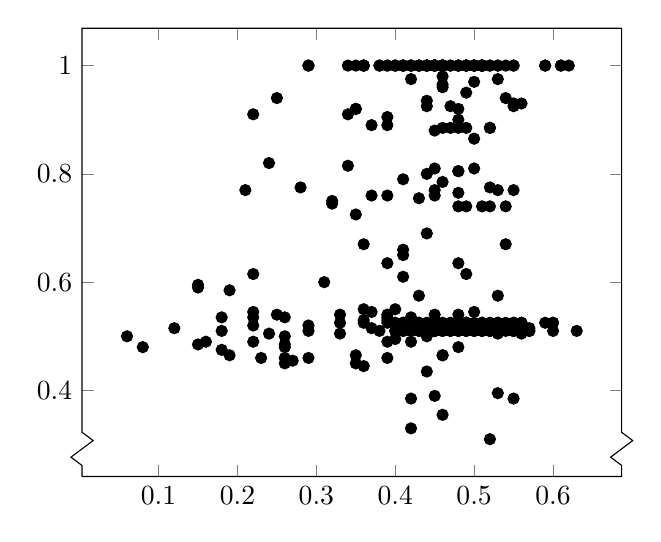
\begin{tikzpicture}
  \begin{axis}[axis y discontinuity=crunch]
  \addplot[scatter src=explicit, only marks]
table {
x y
0.49 0.525
0.4 0.525
0.52 0.525
0.49 0.525
0.47 0.525
0.56 0.525
0.51 0.525
0.5 0.525
0.59 0.525
0.43 0.525
0.41 0.525
0.56 0.525
0.42 0.525
0.46 0.525
0.49 0.525
0.49 0.525
0.41 0.525
0.48 0.525
0.53 0.525
0.43 0.525
0.54 0.525
0.45 0.525
0.45 0.525
0.53 0.525
0.6 0.525
0.55 0.525
0.55 0.525
0.44 0.525
0.45 0.525
0.51 0.525
0.22 0.52
0.28 0.775
0.22 0.545
0.06 0.5
0.29 0.46
0.29 0.52
0.16 0.49
0.15 0.595
0.32 0.745
0.23 0.46
0.18 0.535
0.22 0.615
0.15 0.59
0.33 0.525
0.21 0.77
0.18 0.51
0.35 0.465
0.18 0.475
0.27 0.455
0.26 0.46
0.26 0.48
0.12 0.515
0.26 0.485
0.22 0.535
0.32 0.75
0.39 0.535
0.08 0.48
0.19 0.585
0.15 0.485
0.19 0.465
0.35 0.92
0.37 0.545
0.26 0.5
0.39 0.76
0.31 0.6
0.35 1.0
0.36 0.55
0.25 0.54
0.55 0.925
0.37 0.515
0.39 0.53
0.35 0.92
0.43 1.0
0.35 0.725
0.48 0.9
0.33 0.505
0.39 0.49
0.45 1.0
0.24 0.505
0.45 1.0
0.22 0.49
0.22 0.91
0.36 0.53
0.25 0.94
0.39 0.46
0.49 1.0
0.26 0.535
0.24 0.82
0.46 0.98
0.44 0.5
0.42 1.0
0.52 0.775
0.36 0.445
0.45 0.77
0.26 0.45
0.37 0.89
0.36 0.525
0.29 1.0
0.34 1.0
0.46 0.465
0.41 1.0
0.5 0.97
0.41 1.0
0.42 0.975
0.34 0.91
0.29 1.0
0.41 1.0
0.34 0.815
0.42 0.535
0.42 0.49
0.42 0.515
0.49 1.0
0.39 0.905
0.46 1.0
0.41 0.515
0.33 0.54
0.47 1.0
0.29 0.51
0.46 1.0
0.4 0.55
0.39 1.0
0.43 1.0
0.59 1.0
0.41 0.61
0.5 1.0
0.45 0.53
0.38 1.0
0.46 1.0
0.47 1.0
0.44 1.0
0.41 1.0
0.46 0.965
0.44 1.0
0.51 1.0
0.35 0.45
0.4 1.0
0.45 0.81
0.45 0.54
0.44 0.435
0.44 1.0
0.5 1.0
0.45 1.0
0.36 1.0
0.41 0.79
0.42 1.0
0.46 1.0
0.4 0.495
0.53 0.975
0.45 1.0
0.43 1.0
0.52 1.0
0.5 1.0
0.43 1.0
0.46 0.885
0.39 1.0
0.48 1.0
0.4 1.0
0.53 1.0
0.55 1.0
0.45 1.0
0.51 1.0
0.36 1.0
0.45 1.0
0.36 1.0
0.45 1.0
0.46 0.96
0.4 1.0
0.5 1.0
0.45 1.0
0.36 0.67
0.48 1.0
0.39 0.89
0.48 1.0
0.46 1.0
0.61 1.0
0.49 0.615
0.46 1.0
0.48 0.805
0.49 1.0
0.41 0.65
0.44 0.8
0.46 1.0
0.59 1.0
0.51 1.0
0.39 0.525
0.62 1.0
0.45 1.0
0.61 1.0
0.46 1.0
0.5 1.0
0.47 0.925
0.5 0.81
0.44 1.0
0.48 1.0
0.46 1.0
0.42 0.33
0.42 1.0
0.46 1.0
0.52 1.0
0.51 1.0
0.38 1.0
0.44 1.0
0.46 0.785
0.44 1.0
0.49 1.0
0.42 0.385
0.5 0.545
0.49 0.95
0.41 0.515
0.43 0.755
0.45 0.39
0.41 1.0
0.42 1.0
0.39 0.54
0.49 1.0
0.54 1.0
0.45 1.0
0.48 0.54
0.54 0.67
0.55 1.0
0.36 1.0
0.49 0.885
0.55 0.93
0.53 0.395
0.48 0.48
0.39 0.635
0.51 1.0
0.56 0.93
0.5 0.865
0.52 0.31
0.43 0.575
0.51 1.0
0.44 0.935
0.41 0.66
0.48 0.885
0.52 0.74
0.49 0.51
0.45 0.76
0.54 0.94
0.54 0.74
0.48 0.92
0.44 0.69
0.48 0.765
0.5 0.51
0.48 0.805
0.49 0.74
0.47 0.885
0.46 0.465
0.44 0.925
0.44 1.0
0.45 1.0
0.52 0.885
0.56 0.505
0.49 1.0
0.6 0.525
0.45 0.88
0.52 0.51
0.45 1.0
0.55 0.385
0.45 0.515
0.52 0.885
0.5 1.0
0.46 0.355
0.53 1.0
0.4 0.51
0.45 0.51
0.51 0.74
0.53 0.505
0.47 0.51
0.51 1.0
0.45 1.0
0.53 0.51
0.48 0.74
0.55 0.77
0.44 0.51
0.46 0.51
0.53 0.575
0.41 0.51
0.37 0.76
0.4 0.51
0.48 0.51
0.51 1.0
0.53 0.77
0.52 0.51
0.51 1.0
0.43 0.51
0.57 0.515
0.51 0.51
0.45 0.51
0.48 0.635
0.54 0.51
0.55 0.51
0.57 0.51
0.55 0.51
0.56 0.51
0.52 0.51
0.57 0.51
0.46 0.51
0.53 0.51
0.53 0.51
0.42 0.51
0.63 0.51
0.51 0.51
0.46 0.51
0.53 0.51
0.5 0.51
0.55 0.51
0.6 0.51
0.43 0.51
0.38 0.51
0.49 0.51
0.56 0.51
0.45 0.51
0.51 0.51
0.47 0.51
0.49 0.51
0.42 0.51
0.55 0.51
0.41 0.51
0.45 0.51
0.45 0.51
0.5 0.51
0.52 0.51
0.48 0.51
  };
  \end{axis}
\end{tikzpicture}

%    }
%    \subfloat{
%      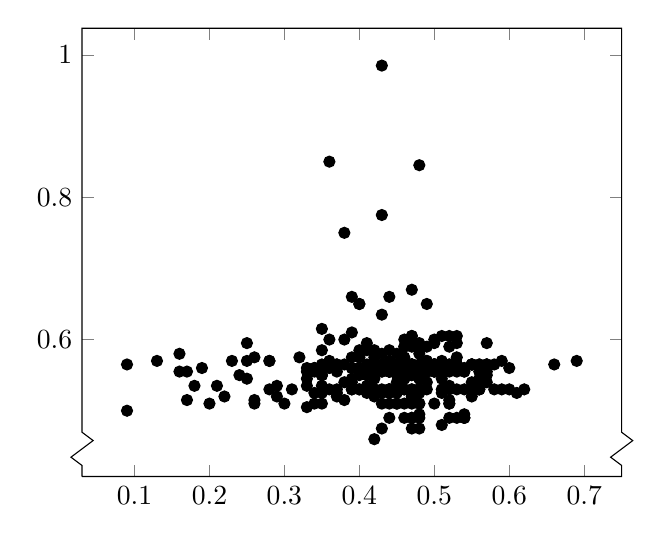
\begin{tikzpicture}
  \begin{axis}[axis y discontinuity=crunch]
  \addplot[scatter src=explicit, only marks]
  table {
x y
0.49 0.565
0.51 0.565
0.52 0.565
0.47 0.565
0.55 0.565
0.43 0.565
0.51 0.565
0.49 0.565
0.5 0.565
0.49 0.565
0.5 0.565
0.45 0.565
0.53 0.565
0.55 0.565
0.51 0.565
0.66 0.565
0.46 0.565
0.57 0.565
0.47 0.565
0.57 0.565
0.47 0.565
0.56 0.565
0.53 0.565
0.53 0.565
0.46 0.565
0.49 0.565
0.43 0.565
0.58 0.565
0.53 0.565
0.42 0.565
0.25 0.57
0.35 0.55
0.25 0.595
0.29 0.52
0.26 0.51
0.28 0.57
0.09 0.5
0.13 0.57
0.25 0.545
0.09 0.565
0.33 0.535
0.34 0.56
0.41 0.565
0.16 0.58
0.34 0.525
0.17 0.515
0.4 0.53
0.4 0.575
0.21 0.535
0.22 0.52
0.35 0.535
0.32 0.575
0.18 0.535
0.24 0.55
0.17 0.555
0.35 0.525
0.38 0.515
0.16 0.555
0.23 0.57
0.19 0.56
0.45 0.53
0.34 0.56
0.29 0.535
0.31 0.53
0.35 0.51
0.46 0.575
0.3 0.51
0.28 0.53
0.48 0.595
0.42 0.52
0.39 0.545
0.34 0.51
0.26 0.515
0.41 0.555
0.4 0.65
0.37 0.555
0.33 0.545
0.4 0.53
0.35 0.615
0.41 0.525
0.36 0.6
0.43 0.525
0.36 0.53
0.49 0.59
0.41 0.535
0.48 0.53
0.28 0.57
0.47 0.525
0.4 0.575
0.47 0.67
0.4 0.555
0.39 0.54
0.41 0.55
0.37 0.52
0.42 0.575
0.56 0.545
0.44 0.555
0.4 0.555
0.34 0.555
0.33 0.505
0.47 0.59
0.47 0.51
0.35 0.55
0.26 0.575
0.38 0.6
0.37 0.565
0.51 0.565
0.35 0.55
0.45 0.555
0.42 0.545
0.43 0.775
0.48 0.53
0.45 0.525
0.33 0.56
0.44 0.66
0.46 0.6
0.39 0.53
0.2 0.51
0.52 0.51
0.45 0.55
0.41 0.595
0.4 0.56
0.42 0.53
0.44 0.56
0.35 0.585
0.42 0.555
0.36 0.57
0.4 0.55
0.36 0.56
0.46 0.555
0.48 0.51
0.43 0.985
0.36 0.85
0.5 0.595
0.44 0.555
0.44 0.585
0.46 0.59
0.44 0.57
0.45 0.54
0.42 0.585
0.55 0.54
0.38 0.54
0.44 0.53
0.46 0.545
0.42 0.53
0.41 0.55
0.33 0.555
0.4 0.56
0.5 0.565
0.37 0.525
0.5 0.6
0.52 0.59
0.43 0.635
0.49 0.555
0.47 0.515
0.48 0.845
0.48 0.585
0.47 0.55
0.44 0.555
0.53 0.56
0.46 0.56
0.45 0.565
0.46 0.56
0.52 0.605
0.43 0.53
0.49 0.65
0.57 0.54
0.49 0.555
0.54 0.56
0.35 0.555
0.44 0.525
0.41 0.585
0.43 0.58
0.39 0.56
0.44 0.555
0.47 0.605
0.49 0.57
0.45 0.58
0.6 0.56
0.47 0.555
0.43 0.555
0.51 0.555
0.55 0.52
0.53 0.555
0.44 0.555
0.49 0.555
0.52 0.535
0.48 0.545
0.4 0.585
0.38 0.75
0.46 0.555
0.53 0.575
0.59 0.57
0.4 0.555
0.54 0.555
0.53 0.595
0.51 0.545
0.45 0.555
0.4 0.555
0.53 0.565
0.39 0.66
0.48 0.545
0.44 0.53
0.49 0.57
0.46 0.59
0.44 0.565
0.4 0.65
0.39 0.575
0.51 0.565
0.37 0.565
0.47 0.555
0.47 0.595
0.48 0.555
0.52 0.565
0.49 0.54
0.56 0.565
0.51 0.56
0.45 0.565
0.57 0.555
0.5 0.555
0.47 0.565
0.48 0.58
0.39 0.56
0.47 0.52
0.45 0.53
0.42 0.555
0.44 0.565
0.53 0.605
0.5 0.555
0.57 0.55
0.46 0.555
0.55 0.565
0.44 0.565
0.5 0.565
0.47 0.55
0.48 0.565
0.51 0.565
0.39 0.61
0.47 0.605
0.43 0.555
0.5 0.565
0.51 0.565
0.46 0.555
0.52 0.555
0.38 0.565
0.57 0.595
0.44 0.565
0.57 0.565
0.55 0.565
0.69 0.57
0.48 0.555
0.51 0.555
0.46 0.545
0.53 0.565
0.49 0.555
0.47 0.565
0.5 0.565
0.42 0.565
0.46 0.565
0.47 0.565
0.51 0.57
0.46 0.57
0.49 0.565
0.5 0.555
0.51 0.605
0.54 0.555
0.35 0.565
0.55 0.565
0.43 0.56
0.56 0.555
0.54 0.49
0.51 0.48
0.44 0.51
0.47 0.49
0.43 0.51
0.54 0.49
0.46 0.49
0.46 0.51
0.48 0.525
0.48 0.475
0.51 0.525
0.47 0.475
0.48 0.51
0.47 0.49
0.53 0.49
0.48 0.495
0.42 0.46
0.54 0.495
0.61 0.525
0.52 0.51
0.52 0.49
0.45 0.51
0.43 0.475
0.44 0.49
0.52 0.515
0.5 0.51
0.45 0.51
0.48 0.49
0.54 0.49
0.62 0.53
0.53 0.53
0.45 0.53
0.45 0.53
0.56 0.53
0.44 0.53
0.52 0.53
0.46 0.53
0.51 0.53
0.58 0.53
0.49 0.53
0.39 0.53
0.6 0.53
0.45 0.53
0.45 0.53
0.56 0.53
0.41 0.53
0.37 0.53
0.56 0.53
0.44 0.53
0.54 0.53
0.46 0.53
0.55 0.53
0.59 0.53
0.48 0.53
0.42 0.53
0.48 0.53
0.47 0.53
0.47 0.53
0.48 0.53
  };
  \end{axis}
\end{tikzpicture}

%    }
%    \subfloat{
%      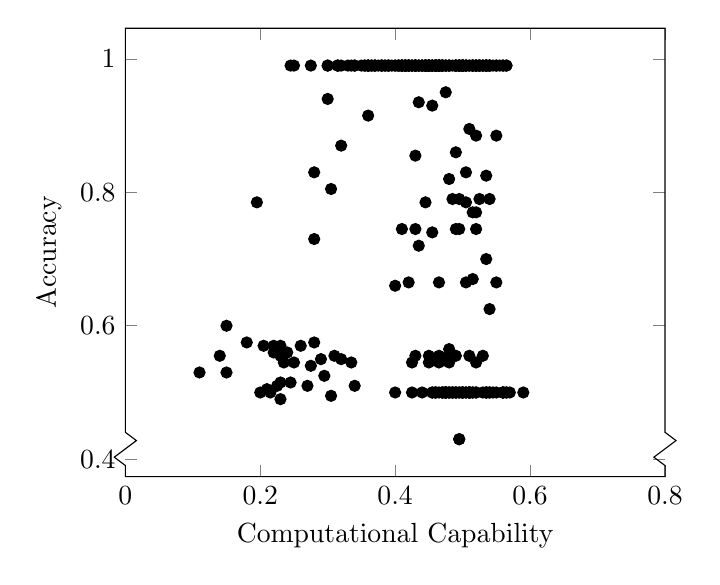
\begin{tikzpicture}
  \begin{axis}
    [
      axis y discontinuity=crunch,
      xmin=0.0, xmax=0.8,
      xlabel=Computational Capability,
      ylabel=Accuracy
    ]
  \addplot[scatter src=explicit, only marks]
  table {
x y
0.475 0.5
0.51 0.5
0.56 0.5
0.47 0.5
0.51 0.5
0.5 0.5
0.51 0.5
0.545 0.5
0.44 0.5
0.46 0.5
0.56 0.5
0.515 0.5
0.535 0.5
0.52 0.5
0.565 0.5
0.505 0.5
0.53 0.5
0.49 0.5
0.48 0.5
0.51 0.5
0.455 0.5
0.56 0.5
0.49 0.5
0.425 0.5
0.455 0.5
0.495 0.5
0.56 0.5
0.54 0.5
0.54 0.5
0.4 0.5
0.27 0.51
0.11 0.53
0.14 0.555
0.18 0.575
0.295 0.525
0.26 0.57
0.31 0.555
0.15 0.53
0.28 0.73
0.22 0.56
0.215 0.5
0.23 0.57
0.23 0.49
0.195 0.785
0.335 0.545
0.23 0.515
0.21 0.505
0.15 0.6
0.245 0.99
0.25 0.545
0.275 0.54
0.36 0.99
0.22 0.57
0.225 0.51
0.24 0.56
0.205 0.57
0.2 0.5
0.235 0.545
0.245 0.515
0.29 0.55
0.34 0.51
0.355 0.99
0.365 0.99
0.32 0.87
0.435 0.72
0.305 0.805
0.42 0.99
0.405 0.99
0.28 0.83
0.3 0.94
0.39 0.99
0.34 0.99
0.36 0.915
0.32 0.99
0.3 0.99
0.37 0.99
0.35 0.99
0.275 0.99
0.37 0.99
0.3 0.99
0.32 0.55
0.315 0.99
0.4 0.66
0.365 0.99
0.305 0.495
0.4 0.99
0.36 0.99
0.315 0.99
0.28 0.575
0.23 0.555
0.36 0.99
0.455 0.99
0.4 0.99
0.41 0.99
0.33 0.99
0.5 0.99
0.41 0.99
0.36 0.99
0.315 0.99
0.38 0.99
0.25 0.99
0.425 0.99
0.39 0.99
0.445 0.99
0.455 0.74
0.385 0.99
0.38 0.99
0.38 0.99
0.405 0.99
0.425 0.99
0.385 0.99
0.465 0.665
0.435 0.935
0.44 0.99
0.335 0.99
0.45 0.99
0.395 0.99
0.495 0.99
0.45 0.99
0.37 0.99
0.53 0.99
0.465 0.99
0.375 0.99
0.415 0.99
0.405 0.99
0.5 0.99
0.42 0.99
0.43 0.99
0.39 0.99
0.515 0.99
0.45 0.99
0.41 0.99
0.435 0.99
0.445 0.99
0.41 0.99
0.47 0.99
0.42 0.99
0.48 0.99
0.43 0.99
0.415 0.99
0.56 0.99
0.45 0.99
0.415 0.99
0.465 0.99
0.53 0.99
0.355 0.99
0.525 0.99
0.51 0.99
0.42 0.99
0.43 0.99
0.465 0.99
0.45 0.99
0.46 0.99
0.48 0.99
0.46 0.99
0.435 0.99
0.545 0.99
0.43 0.99
0.455 0.99
0.48 0.99
0.46 0.99
0.475 0.99
0.43 0.99
0.465 0.99
0.445 0.99
0.34 0.99
0.51 0.99
0.41 0.99
0.415 0.99
0.47 0.99
0.45 0.99
0.485 0.99
0.475 0.99
0.535 0.99
0.44 0.99
0.44 0.99
0.52 0.99
0.415 0.99
0.445 0.99
0.425 0.99
0.505 0.99
0.46 0.99
0.49 0.99
0.565 0.99
0.52 0.99
0.455 0.99
0.45 0.99
0.505 0.99
0.505 0.99
0.52 0.99
0.45 0.99
0.455 0.99
0.465 0.99
0.5 0.99
0.44 0.99
0.465 0.99
0.46 0.99
0.45 0.99
0.47 0.99
0.54 0.99
0.54 0.99
0.445 0.99
0.565 0.99
0.5 0.99
0.45 0.99
0.49 0.99
0.43 0.99
0.55 0.99
0.465 0.99
0.46 0.99
0.515 0.99
0.465 0.99
0.48 0.565
0.525 0.99
0.555 0.99
0.465 0.99
0.54 0.99
0.47 0.99
0.495 0.99
0.415 0.99
0.465 0.99
0.455 0.93
0.5 0.99
0.415 0.99
0.515 0.99
0.41 0.745
0.495 0.99
0.47 0.99
0.53 0.99
0.495 0.99
0.42 0.99
0.45 0.99
0.49 0.99
0.5 0.99
0.495 0.99
0.515 0.99
0.465 0.99
0.5 0.99
0.475 0.95
0.525 0.99
0.505 0.785
0.505 0.99
0.52 0.885
0.43 0.745
0.56 0.99
0.45 0.545
0.525 0.99
0.445 0.99
0.535 0.99
0.535 0.99
0.46 0.99
0.49 0.99
0.52 0.99
0.46 0.99
0.495 0.43
0.525 0.79
0.49 0.99
0.475 0.99
0.535 0.99
0.55 0.99
0.55 0.885
0.49 0.555
0.45 0.555
0.445 0.785
0.48 0.545
0.495 0.745
0.435 0.99
0.535 0.99
0.535 0.825
0.52 0.99
0.54 0.625
0.48 0.555
0.43 0.555
0.43 0.855
0.505 0.83
0.52 0.77
0.505 0.665
0.51 0.555
0.515 0.77
0.535 0.99
0.465 0.545
0.425 0.545
0.535 0.7
0.465 0.555
0.495 0.79
0.515 0.67
0.52 0.545
0.48 0.82
0.49 0.86
0.53 0.555
0.495 0.99
0.485 0.79
0.54 0.79
0.51 0.895
0.55 0.665
0.495 0.43
0.54 0.99
0.49 0.745
0.42 0.665
0.52 0.745
0.535 0.5
0.46 0.5
0.475 0.5
0.5 0.5
0.475 0.5
0.51 0.5
0.485 0.5
0.505 0.5
0.5 0.5
0.48 0.5
0.535 0.5
0.475 0.5
0.46 0.5
0.47 0.5
0.57 0.5
0.52 0.5
0.465 0.5
0.59 0.5
0.495 0.5
0.565 0.5
0.5 0.5
0.49 0.5
0.475 0.5
0.55 0.5
0.485 0.5
0.47 0.5
0.515 0.5
0.485 0.5
0.48 0.5
0.475 0.5
  };
  \end{axis}
\end{tikzpicture}


%    }
%    \subfloat{
%      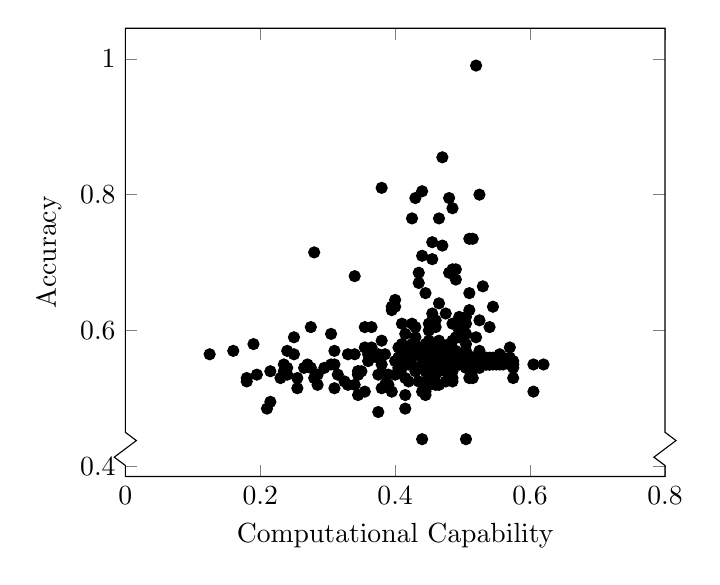
\begin{tikzpicture}
  \begin{axis}
    [
      axis y discontinuity=crunch,
      xmin=0.0, xmax=0.8,
      xlabel=Computational Capability,
      ylabel=Accuracy
    ]
  \addplot[scatter src=explicit, only marks]
  table {
x y
0.62 0.55
0.485 0.55
0.47 0.55
0.525 0.55
0.56 0.55
0.49 0.55
0.44 0.55
0.47 0.55
0.5 0.55
0.48 0.55
0.515 0.55
0.51 0.55
0.55 0.55
0.515 0.55
0.44 0.55
0.5 0.55
0.5 0.55
0.48 0.55
0.54 0.55
0.44 0.55
0.52 0.55
0.5 0.55
0.575 0.55
0.605 0.55
0.535 0.55
0.445 0.55
0.505 0.55
0.47 0.55
0.465 0.55
0.47 0.55
0.275 0.545
0.24 0.545
0.18 0.525
0.215 0.495
0.315 0.535
0.195 0.535
0.24 0.57
0.235 0.54
0.39 0.535
0.25 0.565
0.23 0.53
0.295 0.545
0.305 0.55
0.125 0.565
0.34 0.565
0.16 0.57
0.255 0.515
0.19 0.58
0.345 0.535
0.27 0.55
0.255 0.53
0.215 0.54
0.285 0.535
0.18 0.53
0.31 0.515
0.265 0.545
0.25 0.59
0.21 0.485
0.24 0.535
0.285 0.52
0.325 0.525
0.445 0.58
0.415 0.575
0.485 0.53
0.275 0.605
0.35 0.54
0.375 0.565
0.485 0.525
0.28 0.53
0.365 0.56
0.37 0.565
0.435 0.545
0.345 0.54
0.39 0.52
0.4 0.645
0.33 0.52
0.365 0.605
0.33 0.565
0.345 0.505
0.345 0.535
0.385 0.52
0.41 0.545
0.235 0.55
0.36 0.555
0.305 0.595
0.49 0.59
0.345 0.54
0.28 0.715
0.355 0.605
0.375 0.48
0.44 0.51
0.385 0.535
0.38 0.55
0.45 0.525
0.355 0.575
0.31 0.55
0.355 0.51
0.38 0.81
0.45 0.61
0.415 0.505
0.405 0.555
0.445 0.505
0.425 0.61
0.425 0.58
0.445 0.555
0.385 0.565
0.46 0.615
0.485 0.69
0.36 0.565
0.48 0.575
0.395 0.51
0.485 0.585
0.46 0.55
0.34 0.68
0.4 0.555
0.31 0.57
0.435 0.685
0.435 0.575
0.405 0.56
0.46 0.535
0.505 0.58
0.525 0.8
0.475 0.54
0.395 0.635
0.445 0.51
0.375 0.535
0.43 0.59
0.41 0.56
0.445 0.525
0.425 0.765
0.465 0.64
0.38 0.585
0.47 0.545
0.43 0.605
0.405 0.545
0.435 0.67
0.47 0.725
0.465 0.765
0.48 0.58
0.455 0.565
0.44 0.71
0.46 0.565
0.415 0.53
0.38 0.515
0.42 0.55
0.47 0.855
0.4 0.535
0.365 0.575
0.34 0.52
0.465 0.54
0.405 0.555
0.53 0.665
0.5 0.615
0.48 0.555
0.45 0.54
0.46 0.575
0.5 0.56
0.43 0.795
0.505 0.62
0.435 0.525
0.4 0.635
0.49 0.69
0.415 0.595
0.455 0.73
0.47 0.545
0.485 0.78
0.45 0.52
0.41 0.58
0.47 0.55
0.45 0.555
0.48 0.545
0.445 0.515
0.425 0.57
0.47 0.56
0.49 0.57
0.44 0.805
0.405 0.575
0.44 0.44
0.41 0.61
0.395 0.63
0.465 0.575
0.445 0.57
0.5 0.56
0.46 0.575
0.48 0.795
0.475 0.525
0.515 0.53
0.375 0.56
0.45 0.585
0.445 0.545
0.51 0.63
0.465 0.56
0.455 0.625
0.455 0.545
0.43 0.575
0.445 0.655
0.455 0.705
0.51 0.655
0.455 0.525
0.54 0.605
0.505 0.595
0.48 0.685
0.495 0.6
0.545 0.635
0.495 0.55
0.485 0.61
0.495 0.56
0.455 0.615
0.51 0.735
0.415 0.57
0.475 0.625
0.515 0.735
0.48 0.56
0.56 0.56
0.435 0.565
0.445 0.56
0.405 0.545
0.575 0.555
0.495 0.62
0.42 0.525
0.52 0.59
0.525 0.545
0.52 0.99
0.495 0.55
0.57 0.575
0.49 0.675
0.47 0.56
0.43 0.54
0.46 0.605
0.49 0.55
0.425 0.56
0.465 0.555
0.46 0.52
0.505 0.44
0.52 0.545
0.475 0.55
0.525 0.57
0.405 0.56
0.51 0.56
0.445 0.54
0.525 0.615
0.575 0.53
0.5 0.56
0.51 0.56
0.485 0.54
0.47 0.56
0.465 0.585
0.555 0.565
0.415 0.485
0.465 0.56
0.52 0.56
0.57 0.56
0.555 0.56
0.5 0.56
0.525 0.56
0.47 0.565
0.455 0.53
0.505 0.545
0.475 0.55
0.525 0.56
0.43 0.545
0.55 0.56
0.505 0.61
0.465 0.52
0.495 0.59
0.505 0.57
0.53 0.56
0.5 0.56
0.48 0.55
0.49 0.56
0.535 0.56
0.51 0.545
0.53 0.55
0.52 0.56
0.605 0.51
0.54 0.56
0.51 0.53
0.575 0.545
0.545 0.56
0.51 0.56
0.48 0.56
0.515 0.56
0.465 0.565
0.515 0.56
0.55 0.56
0.48 0.545
0.455 0.56
0.495 0.56
0.49 0.56
0.45 0.56
0.525 0.55
0.515 0.56
0.455 0.56
0.465 0.56
0.485 0.56
0.505 0.56
0.495 0.56
0.5 0.56
0.405 0.56
0.45 0.6
0.485 0.55
0.52 0.55
0.535 0.55
0.515 0.55
0.49 0.55
0.54 0.55
0.51 0.55
0.545 0.55
0.485 0.55
0.575 0.55
0.475 0.55
0.485 0.55
0.445 0.55
0.475 0.55
0.535 0.55
0.57 0.55
0.49 0.55
0.555 0.55
0.51 0.55
0.445 0.55
0.53 0.55
0.54 0.55
0.475 0.55
0.455 0.55
0.51 0.55
0.455 0.55
0.465 0.55
0.485 0.55
0.505 0.55
0.49 0.55
  };
  \end{axis}
\end{tikzpicture}


%    }
%  }
%\end{figure*}

\subsection{Using RBN-reservoirs in solving time-series tasks}

Turns out it works great, as in that 2013 paper.
There seems to be extremely many usable reservoirs, at least for K=2.

\begin{itemize}
  \item Solving the Temporal-Parity task
  \item Solving the Temporal-Density task
\end{itemize}

\subsection{Evolving new RBN-Reservoirs to use existing readout layers}

For some readout layers (4 or so), check if there are multiple acceptable reservoirs for each readout layer.

\begin{itemize}
  \item Show Fitness Graphs with increasing fitness for evolved RBNs
  \item Complexity analysis of RBNs utilizing the same readout layer
\end{itemize}

We see that there are many acceptable RBN-Reservoirs for each readout-layer.
Maybe these RBN-Reservoirs have similar dynamics?


\subsection{Analysis of Dynamics of developed RBN-Reservoirs}

For each group of evolved RBN-Reservoirs (5 or so in each):

\begin{itemize}
  \item Show Computational complexity measure as developed in that 2013 paper
  \item Show transient time for the group
  \item Show Attractor lengths for the group
\end{itemize}


Perhaps the required dynamics are different for the different tasks?
Remember=3 gives different attractors than remember=4. That'd be cool.


Here there'll be an image visualizing one of the groups of evolved RBN-Reservoirs.
Perhaps we can visually identify similarities.
